\section{Architektura}
Architektura platformy je tvořena z několika částí, které jsou navzájem propojeny. Uživatel interaguje s webovou aplikací, která komunikuje s backendem. Backend je tvořen z několika služeb, které komunikují s datovými zdroji dopravců.
\par
\begin{figure}[H]
    \centering
    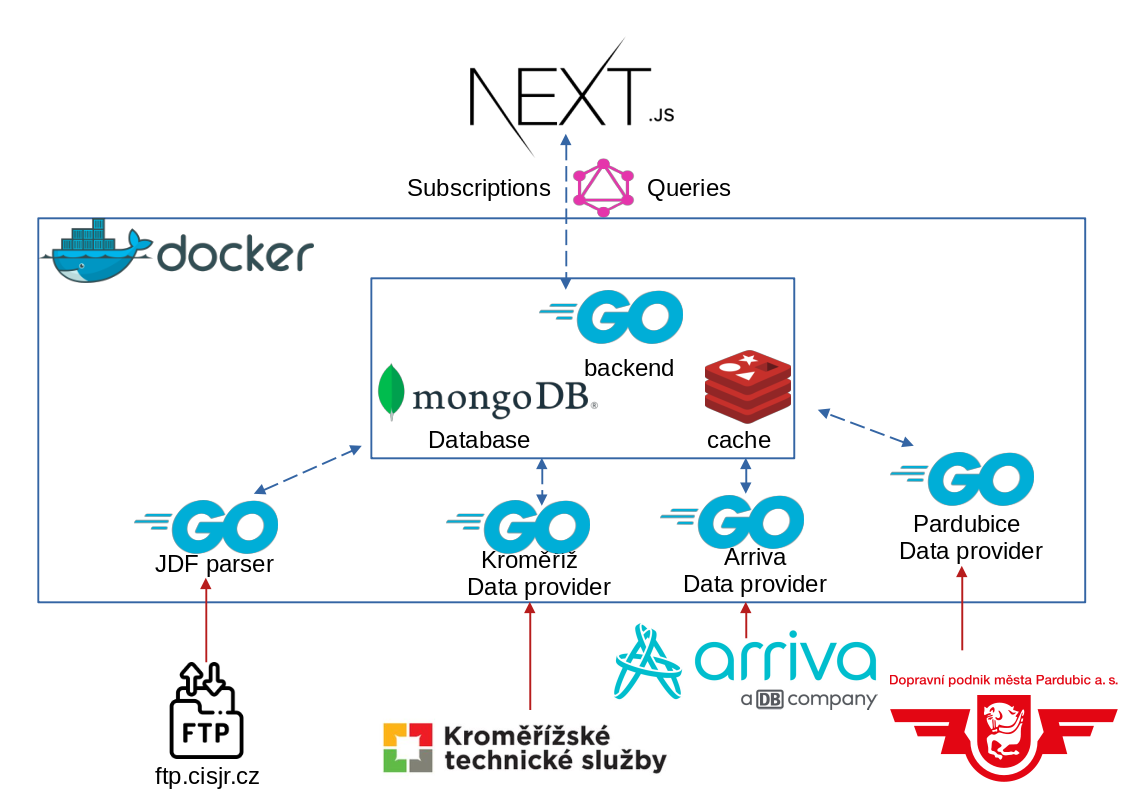
\includegraphics[width=0.75\textwidth]{images/architekturaV5.png}
    \caption{Architektura aplikace}
    \label{architektura}
\end{figure}
\par
Tento projekt je rozdělen do dvou hlavních částí, frontend na frameworku NextJS s využitím programovacího jazyka TypeScript a backend, který je napsán v programovacím jazyce GO.